\section{CMS Overview}
\label{sec:CMS_overview}

In this section there will be an overview about Content Management Systems.

A Content Management System is an application, that provides capabilities for multiple users with different permission levels to manage content, data or information of a website project, or internet application \cite{cms_def}.

Managing content refers to creating, editing, archiving, publishing, collaborating on, reporting, distributing website content, data and information.
So, a CMS is an application that allows creating and publishing content from a central interface. CMSs are often used to run websites containing blogs, news, and shopping. Many corporate and marketing websites use CMSs. CMSs typically aim to avoid the need for hand coding, but may help it for specific elements or entire pages \cite{cms_wiki}. 

A Web CMS may catalog and index content, select or assemble content at runtime, or deliver content to specific visitors in a requested way, such as other languages. Web Content Management System's usually allow client control over HyperText Markup Language - based content, files, documents, and Web hosting plans based on the system depth and the niche it serves.



Nel mondo dei CMS entrano in gioco tre figure principali: lo sviluppatore, l’amministratore e l’utente. Ogni figura svolge un ruolo fondamentale per la vita di un sito web gestito tramite CMS.
Lo sviluppatore è colui che, materialmente, crea il sito web, gestisce le funzionalità e la grafica e effettua il set up per l’amministratore.
L’amministratore è una figura non tecnica (non un programmatore) che gestisce i contenuti del sito: crea, modifica, pubblica e gestisce il materiale da presentare. Egli gestisce i contenuti del sito attraverso un pannello di amministrazione creato ad hoc dallo sviluppatore, all’interno di un’area riservata.
Infine, l’utente è colui che fruisce dei contenuti immessi nel sito dall’amministratore. Non può accedere al pannello di amministrazione e, quindi, non può inserire, modificare o cancellare i contenuti (a volte è possibile commentare i contenuti esistenti).



\begin {figure}[h]
\graphicspath{{images/chapter_cms/}}
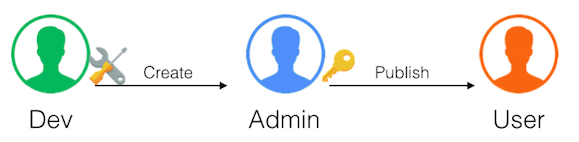
\includegraphics[width=\textwidth]{cms_schema}
\caption{CMS's actors schema}
\end {figure}


